\begin{homeworkProblem}
What is the equation for the entropy of a system consisting of $N$ spin $\frac{1}{2}$ magnetic dipole moments ( $\mu$ ) in an external magnetic field $B$ ? Express your answer in terms of $\mu, \beta$, and $B$. What are the limiting values of the entropy at high temperature and/or weak magnetic field, and at low temperature and/or strong magnetic field. Do these limits make sense?
\begin{callout}{Solution:}
    
    We derived the partition function for a system of $N$ magnetic dipole moments in an external magnetic field:
    $$Z = 2\cosh ^{N}(B\mu \beta)$$
    Mean energy for this is 
    \begin{align*}
        \bar{E} &= - \frac{\partial}{\partial \beta} \ln\left(2\cosh^N(B\mu \beta)\right) \\ 
        &= - N \frac{\partial}{\partial \beta} \ln\left(2\cosh(B\mu \beta)\right) \\ 
        &= - N \left( \frac{2\sinh(\beta \mu B)}{2\cosh(\beta \mu B)} (\mu B) \right) \\ 
        &= N\mu B \tanh(\beta \mu B)
    \end{align*}
    Which means we have entropy 
    $$S = N\ln\left( 2\cosh(\beta \mu B) \right) - N \beta \mu B \tanh(\beta \mu B)$$
    $$s = \frac{S}{N} = \ln\left( 2\cosh(\beta \mu B) \right) -  \beta \mu B \tanh(\beta \mu B)$$

    The plot of this slightly resembles a gaussian curve. 
    \begin{enumerate}[i.]
        \item High temperature/low magnetic field limit: when $\beta\to0$, or $B\to0$ there are many possible configurations of the magnetic moments, which leads to a maxima in entropy.
        \item Low temperature/high magnetic field limit: when $\beta\to\infty$ or $B\to\infty$, entropy drops to zero, i.e. the system becomes totally ordered in one state.
    \end{enumerate}

    \begin{center}
    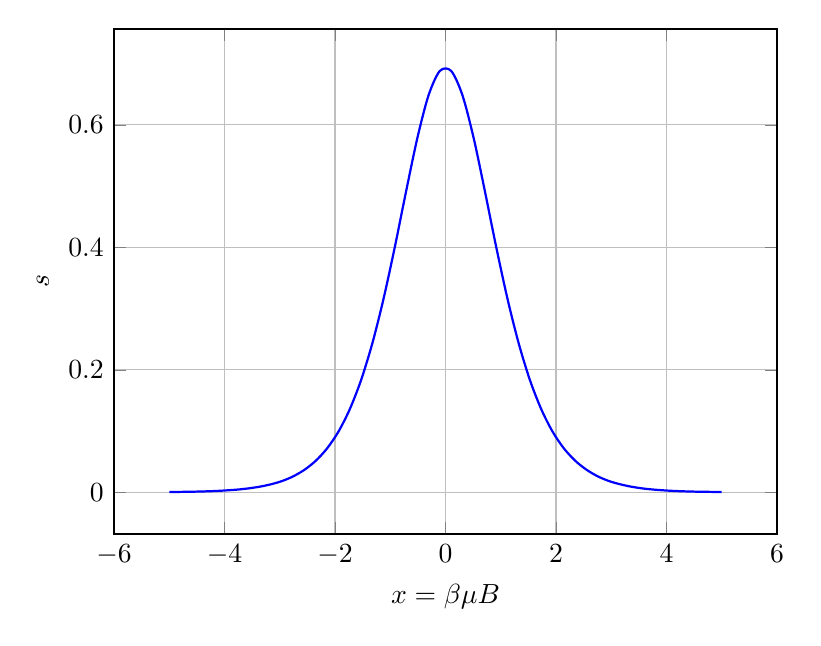
\begin{tikzpicture}
        \begin{axis}[
                width=10cm, height=8cm,
                xlabel={$x = \beta \mu B$},
                ylabel={$s$},
                grid=major,
                legend pos=south east,
                domain=-5:5,
                samples=50,
                thick
                ]

                % Plot for S as a function of x = beta * mu * B
                \addplot[smooth, blue] 
                {ln(2*cosh(x)) - x*tanh(x)};
                %\addlegendentry{$$}

        \end{axis}
    \end{tikzpicture}    
    \end{center}
    
\end{callout}
\end{homeworkProblem}
